\documentclass[eng,oneside]{mgr}
\usepackage{polski}
\usepackage[utf8]{inputenc}
\usepackage[T1]{fontenc}
\usepackage{graphicx}
\graphicspath{ {c:/użytkownicy/nieop/Pulpit} }
\usepackage{subfigure}
\usepackage{rotating}
\usepackage{subfig}
\usepackage{psfrag}
\usepackage{amsmath}
\usepackage{amsfonts}
\usepackage{supertabular}
\usepackage{array}
\usepackage{tabularx}
\usepackage{hhline}
\usepackage{showlabels}
\usepackage{indentfirst}
\usepackage{caption}
\usepackage{listings}
\renewcommand{\lstlistingname}{Kod źródłowy}
\usepackage{courier}
\lstset{basicstyle=\footnotesize\ttfamily,breaklines=true,captionpos=b}
\captionsetup[lstlisting]{belowskip=\baselineskip,justification=centering}

\title{Rozpoznawanie znaków tekstowych drogowych w systemie pomocy osobom niewidomym}
\engtitle{The text road signs recognition in the system of helping visually-impaired people}
\author{Karolina Raczyńska}
\supervisor{dr inż. Łukasz Jeleń}
\date{09.12.2016}
\field{Automatyka i Robotyka (AIR)}
\specialisation{Technologie Informacyjne w Automatyce (ART)}
\begin{document}
\maketitle
\tableofcontents 

\chapter{Wstęp}
Postęp techniczny w XXI wieku sprawił, że technologie informatyczne wkroczyły już do wielu sfer naszego życia, oferując co raz to nowsze i lepsze rozwiązania. Od dziesiątek lat firmy IT skupiają się na tym, aby dotrzeć nie tylko do statystycznego klienta, ale też do tych szczególnych, ze specjalnymi potrzebami. Pojawiają się narzędzia, które pomagają funkcjonować w społeczeństwie ludziom, którzy postrzegają świat nieco innymi zmysłami - przez swoją niepełnosprawność. W świecie gdzie tysiące ludzi wpatruje się w swoje smartfony, dla ludzi niewidomych to doświadczenie jest zgoła inne. Celem producentów urządzeń mobilnych staje się rozciągnięcie swojej oferty, dla ludzi również niepełnosprawnych sensorycznie - niedowidzących czy słabosłyszących. Na rynek zaczynają napływać aplikacje, które pomagają ludziom niedowidzącym czy całkowicie niewidzącym korzystać z telefonów komórkowych. Istnieją aplikację czytające wiadomości tekstowe, nadesłane do posiadacza telefonu, a także takie które odwrotnie, zamieniają tekst mówiony na wiadomość. Pojawiają się możliwości dostosowania właściwości telefonu do potrzeb konsumenta, takie jak np. nakładki na system w telefonie, które powiększają czcionkę. Popularne jest wybieranie głosowe, które ułatwia korzystanie z telefonu nie tylko ludziom z problemami ze wzrokiem, ale też osobom starszym. 
\par W Instytucie Nauki w Georgii grupa badaczy poczyniła wielki krok w kierunku pomocy ludziom niepełnosprawnym - stworzyła aplikację BrailleTouch, która  pozwala wprowadzać tekst do smartfona, bez używania wzroku. Urządzenie musi być trzymane horyzontalnie, po obu stronach znajdują się wtenczas po trzy przyciski. Korzystając z sześciu palców, trzyma się je nad przyciskami, co nie wymaga od użytkownika przemieszczania palców po ekranie. Właściwe konfiguracje naciśnięć tych przycisków, tworzą wszystkie litery alfabetu, a także znaki specjalne. Jak nazwa aplikacji wskazuje idea ta jest oparta na alfabecie Braille'a, wystarczy dotykać odpowiednie kombinacje przycisków, a do pola tekstowego zostaje wprowadzony właściwy znak. Aplikacja jest też przygotowana na obsługę błędów. Informuje użytkownika o błędach jakie popełnił, np. przez wiadomość głosową czy wibracje \cite{touch}. 
\par Dąży się do tego aby doświadczenia sensoryczne ludzi niepełnosprawnych wizualnie, korzystających z urządzeń mobilnych były pełniejsze. W tym celu stosuje się właśnie wibracje, czy komunikaty głosowe. Właśnie te proste właściwości, wbudowane w każdym telefonie, a także ogrom algorytmów wspierających przetwarzanie obrazu, zachęcają do pisania aplikacji wspierających osoby niewidome i niedowidzące. Chce się, aby dzięki smartfonom te osoby mogły "patrzeć", korzystając jednak z innych zmysłów. Ważnym zastosowaniem telefonów w tym aspekcie jest pomoc osobom niewidomym w zachowaniu bezpieczeństwa, wykorzystanie urządzenia mobilnego jako elektronicznego przewodnika takiej osoby, ostrzegającego ją o ewentualnych zagrożeniach, które mogą ją spotkać na drodze, np. informacja o tym, że zbliża się do strefy ruchu, gdzie może napotkać samochód, tudzież, że powinna zwrócić uwagę na roboty drogowe czy inne utrudnienia w ruchu. Rozpoznawanie otoczenia, w którym dana osoba się znajduje ma także wartość informacyjną - powiadamia, dla przykładu o nazwie ulicy na której się znajduje, jeżeli w okolicy znajduje się tabliczka z ową nazwą. Taka informacja zwrotna pod wpływem analizy otoczenia, przy wykorzystaniu urządzenia mobilnego będzie tematem niniejszej pracy inżynierskiej.

\section{Cel i zakres pracy}
Celem niniejszej pracy było stworzenie systemu wsparcia dla osób niewidomych i niedowidzących. Zdecydowano się zawęzić zakres pracy do napisania aplikacji mobilnej, wspierającej takie osoby. Aplikacja ta miała być na tyle intuicyjna i łatwa w obsłudze, aby osoby te mogły z niej korzystać bez większych problemów. Kolejnym celem było opisanie jej, ze szczególnym zwróceniem uwagi na algorytmy użyte przy jej powstawaniu i przeanalizowanie ich działania, a także naświetlenie pewnych informacji na temat środowiska Android. Aplikacja powinna działać na jak najmniejszej liczbie urządzeń, starając się wszystkie swoje funkcje, czyli zrobienie zdjęcie, przetworzenie go, zaprezentowanie informacji zwrotnej użytkowniki, zawrzeć w jednym urządzeniu mobilnym - telefonie z systemem operacyjnym Android, który, na dzień dzisiejszy, jest najbardziej popularnym systemem na rynku. Koniecznym warunkiem ma być jednak to, że ów telefon musi posiadać sprawny aparat i głośnik. Główną funkcjonalnością aplikacji miało być przetwarzanie zdjęć, na których znajdowały się tekstowe znaki drogowe na komunikat głosowy. Dzięki czemu poruszanie się po ulicy ludzi, mających trudność z czytaniem drogowych znaków tekstowych, stałoby się łatwiejsze, a przede wszystkim bezpieczniejsze, z uwagi na to, że tego typu znaki przekazują wiadomości istotne dla podróży niezagrażającej ludzkiemu zdrowiu, a także życiu. Pomysł niniejszej pracy powstał jako dopełnienie większego systemu wsparcia dla osób niewidomych, składającego się na rozpoznawanie tekstu mówionego i przetwarzanie elektrowibracji, stanowiącego rozwinięcie projektu zespołowego "Sztuczne Oko". Projekt ów opierał się na użyciu telefonu z aparatem, który robił zdjęcie i przetwarzał je na krawędzie, kompresował i przesyłał na Raspberry Pi, a tam konwertowane było na sygnał audio, który prowokował elektrowibracje na panelu dotykowym, ładowanym przez przetwornicę, w miejscu gdzie zarejestrowano położenie palca. Elektrowibracje te miały imitować uczucie szorstkości pod palcami, doprowadzając do możliwości "widzenia" krawędzi odczytanych ze zdjęcia, opuszkami palców.

\section{Struktura pracy}
Praca podzielona jest na siedem rozdziałów, pierwszy to Wstęp, wprowadzający czytelnika w temat pracy, określający jej cel i zakres. Ostatni to Zakończenie, gdzie podsumowuje się całą pracę i stwierdza czy jej cele zostały spełnione. 
\par Drugi rozdział przedstawia podstawy teoretyczne, które zostały wykorzystane przy tworzeniu aplikacji. Przedstawiono podstawowe zagadnienia z dziedziny przetwarzania obrazu, opisano użyte algorytmy, ich działanie, zalety oraz wady, a także to jak prezentują się przy innych algorytmach rozwiązujących ten sam problem.
\par W trzecim rozdziale zawarto architekturę stworzonego systemu, zaprezentowano diagramy UML: klas oraz przypadków użycia. Opisano strukturę programu oraz działanie poszczególnych klas, jakie operacje wykonywane są na obiektach tych klas, a także powiązania między nimi. 
\par W czwartym rozdziale odniesiono się do implementacji programu. Przedstawiono środowisko w którym został napisany i zaprezentowano jego najważniejsze komponenty. Pojawiły się również przykłady kodu, wycięte z kodu źródłowego aplikacji, wraz z wytłumaczeniem ich znaczenia oraz celem wykorzystania. Opisano również zewnętrzne biblioteki, które zostały użyte.
\par W piątym rozdziale pokazano działanie aplikacji, dołączono screeny ekranu urządzenia mobilnego, na którym aplikacja była testowana. Dołączono opis wszystkich funkcjonalności oraz możliwych widoków. 

\chapter{Przetwarzanie obrazu}
Obraz to między innymi źródło informacji - nie tylko wzrokowej. Aby uzyskać dane, które są w nim zapisane, należy go odpowiednio przetworzyć. W dziedzinie nauki, jaką jest przetwarzanie obrazów, wyróżniamy kilka etapów działania. Uproszczony schemat został przedstawiony na rysunku poniżej.
\begin{figure}[htbp]
\centering
\captionsetup{justification=centering}
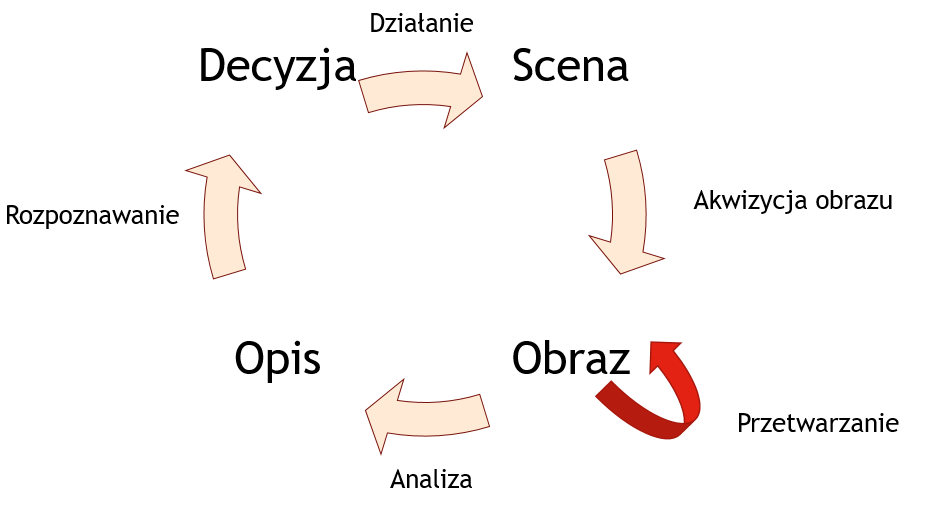
\includegraphics[scale=0.5]{cyklprzetwarzania.png}
\caption{Schemat cyklu przetwarzania obrazu \\ 
źródło: opracowanie własne na podstawie \cite{rysunek}}\par\medskip
\end{figure}
\par Poniżej zostały omówione poszczególne etapy.
\begin{enumerate}
\item 	\textbf{Akwizycja obrazu} – zamiana energii świetlnej od każdego punktu sceny na sygnał elektryczny, czyli zbieranie danych o każdym pikselu. Scena jaką obserwujemy jest funkcją ciągłą, przy przetwarzaniu jej na obraz cyfrowy, pewna część danych zostaje stracona. Typowo korzysta się z dwóch sposobów pozyskiwania sygnały dyskretnego z sygnału ciągłego i jest to: kwantyzacja oraz próbkowanie. Kwantyzacja jest to pobieranie danych w funkcji wartości funkcji – w zależności od niej przyporządkowuje się próbkę do odpowiedniego przedziału, czyli kwantu, natomiast próbkowanie polega na zbieraniu danych w funkcji czasu.
\item 	\textbf{Przetwarzanie obrazu} – na ten etap składa się wstępna obróbka obrazu, operacje takie jak: zmniejszenie obrazu, eliminacja zakłóceń, filtracja wstępna, której celem jest wyeksponowanie na obrazie ważnych cech, takich jak krawędzie lub duże jednokolorowe obiekty. Do tego celu stosuje się np. transformację obrazu kolorowego na skalę odcieni szarości, tudzież progowanie, w celu uzyskania obrazu binarnego, w którym piksele przyjmują jedynie jedną z dwóch wartości.
\item 	\textbf{Analiza obrazu} – wydobycie wcześniej wyeksponowanych cech, w celu ich późniejszego rozpoznania, już nie jako kształtu ale jako konkretnej informacji. Wynikiem tego etapu nie jest już obraz, a dane w postaci liczbowej lub statystycznej.
\item 	\textbf{Decyzja} – rozpoznanie obrazu, zanalizowanie cech, pozyskanie informacji, a przede wszystkim klasyfikacja \cite{obrazy}.
\end{enumerate}
\par Wszystkie te etapy mają miejsce w systemie wizyjnym do którego można zaliczyć np. komputer, telefon, aparat fotograficzny, a do jego podstawowych funkcji należy:
\begin{itemize}
\item Przyjęcie obrazu,
\item zapisanie obrazu,
\item właściwa obróbka obrazu,
\item wyświetlenie obrazu \cite{wizja};
\end{itemize}

\section{Przetwarzanie do skali szarości}
RGB, jest modelem przestrzeni barw, w którym każdy piksel opisują trzy wartości: R - intensywność koloru czerwonego, G - intensywność koloru zielonego oraz B - intensywność koloru niebieskiego. Obraz w odcieniach szarości to obraz w którym procentowy udział każdej z tych trzech instancji jest równy. Aby uzyskać taki wynik należy przeprowadzić pewne modyfikacje na wartościach pikseli. Przyjmuje się, że p to piksel wynikowy operacji przetwarzania do skali szarości. Najbardziej znane są trzy algorytmy:
\begin{itemize}
\item Desaturacja(ang. Desaturation) – metoda ta polega na tym, że z trzech wartości: intensywności koloru czerwonego, zielonego oraz niebieskiego w pikselu, zostaje wybrana wartość największa oraz najmniejsza, a wynikiem transformacji jest średnia arytmetyczna tych dwóch wartości.
\begin{equation}
p=\frac{max(R,G,B) + min(R,G,B)}{2}
\end{equation}
\item Średnia (ang. Average) – metoda ta, najprostsza, dzieli sumę wartości intensywności trzech kolorów przez trzy.
\begin{equation}
p=\frac{R + G + B}{3}
\end{equation}
\item Jasność (ang. Luminance) – metoda również opierająca się na średniej, ale w tym wypadku jest to średnia ważona. Ludzki wzrok jest najbardziej czuły na kolor zielony, właśnie dlatego intensywność zieleni ma największą wagę. Wyjściowy piksel przyjmuje wartość \cite{grayscale}:
\begin{equation}
p={0.21R + 0.72G + 0.07B}
\end{equation}

\end{itemize} \newpage
\par Wyniki poddania obrazu powyższym transformacją zostały przedstawione na Przykładzie 2.2.
\begin{figure}[hbtp]
\centering
\captionsetup{justification=centering}
\subfigure[Obraz oryginalny]{
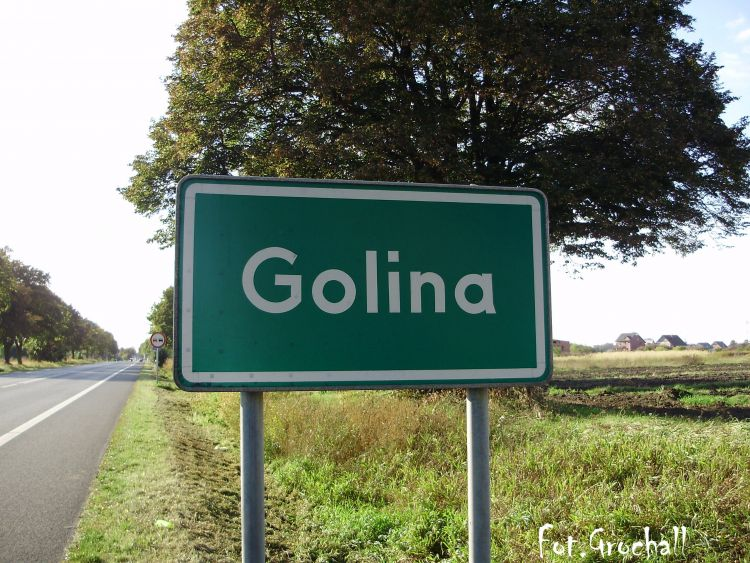
\includegraphics[scale=0.25]{golinatlo.jpg}
}
\quad
\subfigure[Obraz po poddaniu desaturacji]{
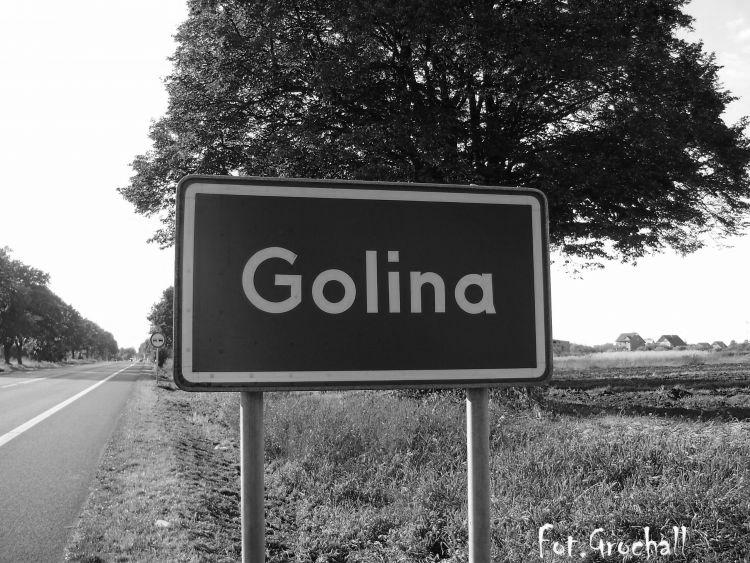
\includegraphics[scale=0.25]{golinalightness.jpg}
}
\quad
\subfigure[Obraz po poddaniu uśrednieniu]{
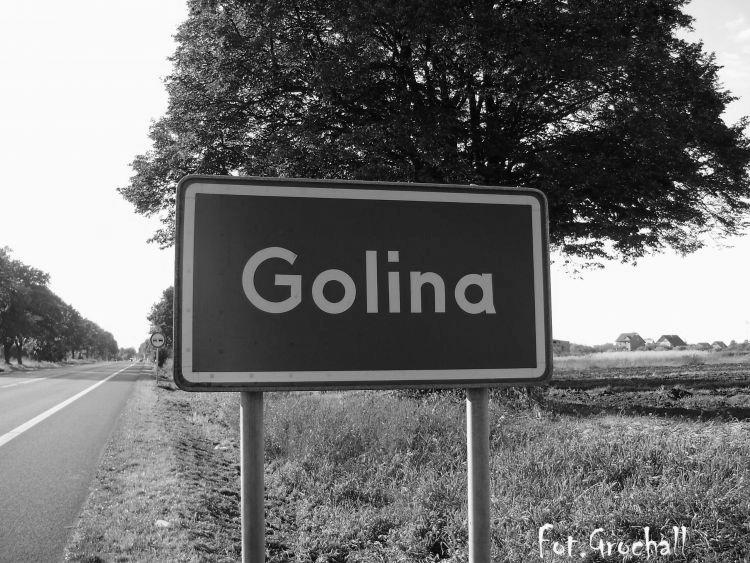
\includegraphics[scale=0.25]{golinaaverage.jpg}
}
\quad
\subfigure[Obraz po poddaniu operacji jasność]{
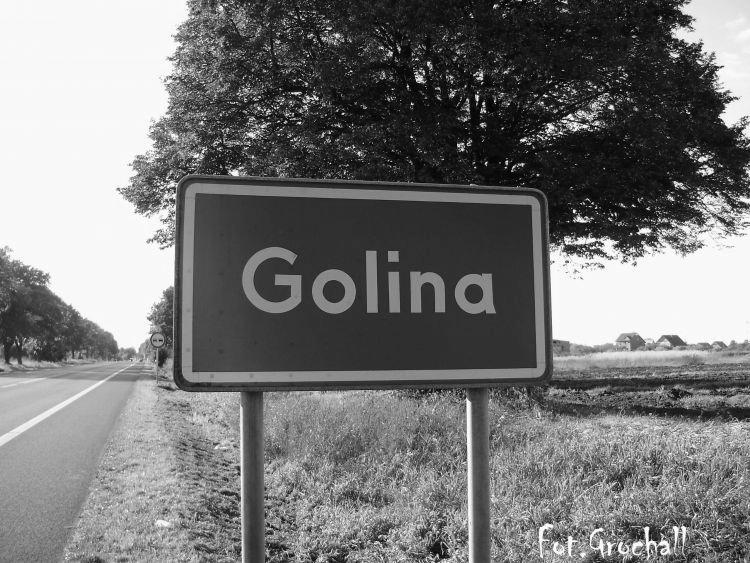
\includegraphics[scale=0.25]{golinaluminance.jpg}
}
\renewcommand\figurename{Przykład}
\caption{Wynik przetwarzania obrazu na odcienie szarości\\ 
źródło: opracowanie własne}
\end{figure}
\section{Binaryzacja}
Binaryzacja to operacja punktowa. Wynikiem tej operacji jest obraz binarny, czyli taki, w którym każdy z pikseli przyjmuje tylko jedną z dwóch wartości. Ideą tego zabiegu jest wyodrębnienie obiektu od tła przez nadanie pikselom, tych dwóch instancji, różnych wartości. Wejściowym obrazem jest zazwyczaj obraz przetworzony do skali szarości, którego piksele przyjmują wartości od 0 do 255. Najczęściej stosowaną metodą klasyfikacji piksela do jednej z dwóch klas jest progowanie – sprawdzenie czy wartość piksela przekracza zadany próg czy też nie i w zależności od wyniku tego zdania logicznego – przypisanie odpowiedniej wartości. Dla progu $T$, początkowej wartości piksela $I(i,j)$ i wartości piksela po transformacji $Y(i,j)$, gdzie $i$ to współrzędna pozioma, a $j$ to współrzędna pionowa piksela na obrazie, mamy \cite{prog}:
\begin{equation}
I(i,j) < T \longmapsto Y(i,j) = 0 
\end{equation}
\begin{equation}
I(i,j) \geq T \longmapsto Y(i,j) = 1 
\end{equation}
Zasadniczą trudnością tego podejścia jest celne dobranie wartości progowej $T$. Aby wybrać odpowiednią wartość progu można zastosować jeden z poniżej zamieszczonych sposobów:
\begin{itemize}
\item \textbf{Na podstawie histogramu} - należy użyć histogramu poziomów szarości analizowanego obrazu. Histogram to graficzna reprezentacja rozkładu empirycznego cechy. Na wykresie zaprezentowany jest jako bloczki o odpowiedniej wysokości w zależności od liczby pikseli przyjmujących wartości z danego zakresu \cite{histogram1}. Następnie, w przypadku gdy histogram jest dwumodalny, to wartość progową wybiera się z pomiędzy dwóch maksimów lokalnych. Gdy ma się do czynienia z mniej szczególnym przypadkiem zastosowanie tej metody może spowodować przekłamania w wyborze progu \cite{histogram}.
\item \textbf{Zastosowanie dwóch wartości progowych} - rozważa się progowanie z dwoma wartościami $T_1 > T_2 > 0$. Jeżeli wartości piksela znajduje się pomiędzy wartościami $T_1$ i $T_2$ przyporządkowuje mu się wartość 0, w przeciwnym wypadku 1. Tego typu podejście ma sens, kiedy tło obrazu jest o różnych poziomach szarości. Można też uśrednić poziom szarości tła. Podobnym sposobem jest zastosowanie histerezy, tutaj analizuje się jednak jeszcze sąsiednie piksele \cite{dwaprogi}. 
\item \textbf{Automatyczny dobór wartości progowej} - próg wybierany jest programowo, korzystając z pewnego algorytmu. Te metody bazują na pewnych założeniach, histogram musi być bimodadalny, obiekty muszą być w kolorach przeciwnych do kolorów tła. Do metod automatycznych zalicza się przedstawioną szerzej metodę Otsu \cite{auto}.
\end{itemize}

\subsection{Metoda Otsu} 
Metoda Otsu należy do rodziny metod optymalnych względem pewnej funkcji kryterialnej. W tym przypadku ową funkcja kryterialną jest wariancja wewnątrzklasowa oraz międzyklasowa. Metoda ta jest bardzo prosta, w uogólnieniu używa momentów zerowego oraz pierwszego stopnia histogramu obrazu.
\par Pierwszym etapem poszukiwania wartości progowej metodą Otsu jest normalizacja histogramu obrazu w skali szarości. Zakłada się, że piksele przyjmują wartości z $L$ poziomów, a do każdego i-tego poziomu jest przydzielana $n_i$ liczba pikseli. Przyjmując, że $N$ to liczba wszystkich pikseli obrazu, rozkład prawdopodobieństw $p_i$ tego histogramu przedstawiony jest następująco:
\begin{equation}
 p_i = \frac{n_i}{N} \hspace{1cm}
 p_i \geq 0, \sum_{i=1}^L p_i = 1 
\end{equation}
\par Następnym krokiem jest dychotomia pikseli, czyli podział wszystkich elementów na dwie klasy względem pewnego progu $t$. Wtenczas piksele, które przyjmują wartości mniejsze od zadanej wartości progowej $t$ zostaną sklasyfikowane do klasy $K_0$, a te większe do klasy $K_1$. Wtedy prawdopodobieństwo $\omega_0$ oraz $\omega_1$ tego, że badany piksel zostanie przypisany do danej klasy jest określone wzorami:
\begin{equation}
\omega_0 = Pr(K_0)=\sum_{i=1}^t p_i = \omega(t)\hspace{1cm}
\end{equation}
\begin{equation}
\omega_1 = Pr(K_1)=\sum_{i=t+1}^L p_i = 1 - \omega(t)
\end{equation}
\par Średnia wartość piksela $mu_0$ oraz $mu_1$ przyjmowana w klasie określona została w poniższych wzorach:
\begin{equation}
\mu_0=\sum_{i=1}^t Pr(i|K_0)=\sum_{i=1}^t \frac{ip_i}{\omega_0}=\frac{\mu(t)}{\omega(t)}
\end{equation}
\begin{equation}
\mu_1=\sum_{i=t+1}^L iPr(i|K_1)=\sum_{i=t+1}^L \frac{ip_i}{\omega_1} = \frac{\mu_T-\mu(t)}{1-\omega(t)}
\end{equation}
\par Gdzie:
\begin{equation}
\omega(t)=\sum_{i=1}^t p_i
\end{equation}
\begin{equation}
\mu(t)=\sum_{i=1}^t ip_i
\end{equation}
\par Powyższe wartości są skumulowanymi momentami zerowego oraz pierwszego stopnia obrazu dla wartości progowej równej $t$. A średnia z wartości pikseli na całym obrazie może zostać zapisana wzorem:
\begin{equation}
\mu_T = \mu(L) = \sum_{i=1}^L ip_i
\end{equation}
\par Niezależnie od wyboru wartości parametru $t$, prawdziwe są równania:
\begin{equation}
\omega_0\mu_0+\omega_1\mu_1=\mu_T, \hspace{1cm} \omega_0+\omega_1=1. 
\end{equation}
\par Wariancje obu klas można przedstawić następująco:
\begin{equation}
\sigma_0^{2}=\sum_{i=1}^t {(i-\mu_0)}^2 Pr(i|K_0)=\sum_{i=1}^t {(i-\mu_0)}^2 \frac{p_i}{\omega_0}
\end{equation}
\begin{equation}
\sigma_0^{2}=\sum_{i=t+1}^t {(i-\mu_1)}^2 Pr(i|K_1)=\sum_{i=t+1}^L {(i-\mu_1)}^2 \frac{p_i}{\omega_1}
\end{equation}
\par W kolejnym etapie należy sprawdzić czy wartość zmiennej $t$ jest wartością optymalną względem funkcji kryterialnej. Funkcją kryterialną, jak wcześniej wspomniano jest:
\begin{itemize}
\item Wariancja wewnątrzklasowa, dąży do minimalizacji,
\begin{equation}
\lambda=\frac{\sigma_B^2}{\sigma_W^2}, \hspace{0.5cm} \sigma_W^2 = \omega_0\sigma_0^2 + \omega_1\sigma_1^2, \hspace{0.5cm} \sigma_B^2 = \omega_0\omega_1{(\mu_1-\mu_2)}^2 
\end{equation}
\item Wariancja międzyklasowa, dąży do maksymalizacji.
\begin{equation}
\kappa=\frac{\sigma_T^2}{\sigma_W^2}, \hspace{0.5cm} \sigma_T^2 = \sum_{i=1}^L {(i-\mu_T)}^2 p_i 
\end{equation}
\end{itemize}
\par Teoria ta intuicyjnie zgadza się z pożądanym efektem działania algorytmu. Chce się aby wartości pikseli w klasach były do siebie jak najbardziej zbliżone, a między klasami występowała jak największa różnica.
Kryterium jakie stosuje się do optymalizacji wartości $t$ jest łączna wariancja poziomów $\eta$. Parametr jest optymalny, jeżeli $\eta$ przyjmuje wartość jak największą, tym samym wariancja wewnątrzklasowa. Wartość ta będzie zerowa jedynie w przypadku gdy wszystkie piksele obrazu zostaną zakwalifikowane tylko do jednej z klas, jednak jest to sprzeczne z celem działania algorytmu, więc w tym kontekście maksimum zawsze istnieje.
\begin{equation}
\eta=\frac{\sigma_B^2}{\sigma_T^2}, \hspace{0.5cm} 
\end{equation}
\par Zaletą tej metody jest jej prostota – korzysta się jedynie z momentów zerowego i pierwszego rzędu, a także stabilność – optymalny próg jest wybrany automatycznie, nie bazuje na zróżnicowaniach (takich jak lokalne zbiory pikseli o niskich lub wysokich wartościach), skupia się na globalnych właściwościach obrazu, histogramie. Ważną cechą jest też uniwersalność metody, dzięki, której można ją wykorzystywać w różnych dziedzinach analizy obrazu. Może służyć do binaryzacji, jak wykorzystano w projekcie, wykorzystywana jest też przy progowaniu \cite{binaryzacja}. Wadą tej metody jest możliwość błędu poprzez wybranie niewłaściwej wartości początkowej $t$. 
\par Wynik poddania obrazu powyższej transformacji został przedstawiony na Przykładzie 2.3.
\begin{figure}[htbp]
\centering
\subfigure[Obraz oryginalny]{
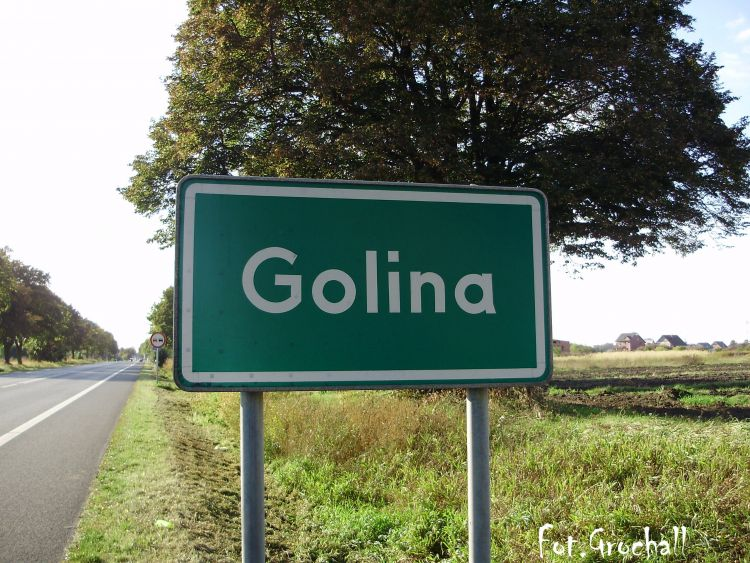
\includegraphics[scale=0.25]{golinatlo.jpg}
}
\quad
\subfigure[Obraz po progowaniu]{
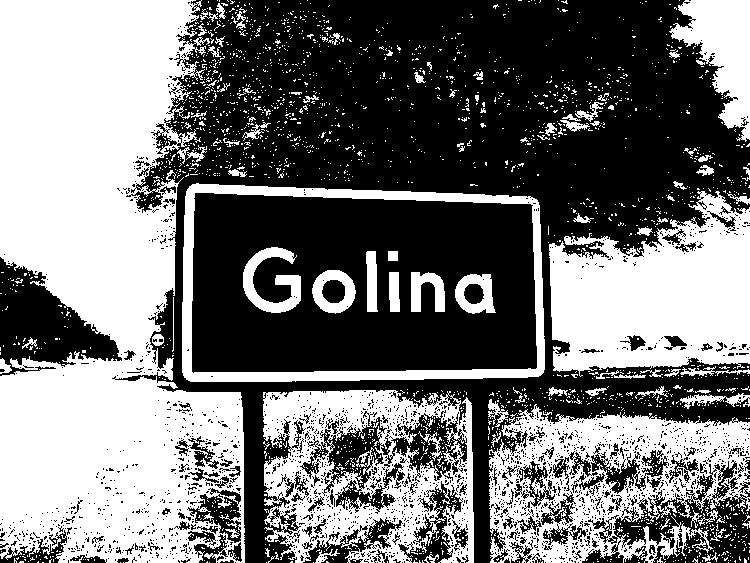
\includegraphics[scale=0.25]{golinaotsu.jpg}
}
\renewcommand\figurename{Przykład}
\caption{Wynik progowania obrazu metodą Otsu\\ 
źródło: opracowanie własne}
\end{figure}

\section{Wykrywanie krawędzi}
Przetwarzanie obrazów opiera się na wydobywaniu z obrazu takich cech, które są istotne przy późniejszej analizie i identyfikacji obiektów na nim zawartych. Jedną z takich cech jest krawędź, czyli znaczna lokalna zmiana w intensywności obrazu, związana z brakiem ciągłości w intensywności obrazu lub w pierwszej pochodnej intensywności obrazu. Występują dwa rodzaje takiej zmiany ciągłości:
\begin{enumerate}
\item \textbf{Nieciągłość skokowa} - intensywność obrazu zmienia się z jednej wartości w drugą i przez jakiś czas tą wartość utrzymuje, przypomina odpowiedź skokową, na obrazie może być to moment styku dwóch obiektów;
\item \textbf{Nieciągłość liniowa} - intensywność obrazu zmienia się z jednej wartości w drugą lecz w krótkim okresie czasu do niej powraca, przypomina odpowiedź impulsową, na obrazie może to być przerwanie w obiekcie; 
\end{enumerate}
\par W praktyce jednak tego typu krawędzie zdarzają się dość rzadko, krawędzie nie są aż tak wyraziste i skok przypomina bardziej rampę, a linia - dach \cite{krawedz}.

\par Wykrywanie krawędzi to przede wszystkim rozpoznawanie znacznych zmian w obrazie, jest to mocno związane z wyznaczaniem maksimum pierwszej pochodnej. 
\par Gradient jest miarą zmiany, wektorem, który wskazuje kierunki i szybkość wzrostu wartości, to dwuwymiarowy odpowiednik pierwszej pochodnej. W obrazie zmianą jest różnica w intensywności koloru. To właśnie on jest bazą większości algorytmów wykrywających krawędzie. Do operatorów gradientowych należy: operator Robertsa, gdzie krawędź to tutaj maksimum pierwszej pochodnej gradientu, operator Prewitta, który opiera się na wygładzeniu obrazu w kierunku ortogonalnym do kierunku w którym wyznaczana jest pochodna oraz operator Sobela, gdzie krawędź jest również wyznaczana przez maksimum pierwszej pochodnej i używany jest jednowymiarowy filtr uśredniający. Gradient obrazu dany jest wzorem:
\begin{equation}
\nabla f = \binom{g_x}{g_y} = \binom{\frac{\delta f}{\delta x}}{\frac{\delta f}{\delta y}}
\end{equation} 
\par Gdzie:
\par $g_x $- gradient w kierunku x,
\par $g_y $- gradient w kierunku y

\par Kierunek zmian można wyliczyć z poniższego wzoru:
\begin{equation}
\theta = \tan^{-1} \binom{g_x}{g_y}
\end{equation}
\par Etapy wykrywania krawędzi:
\begin{enumerate}
\item \textbf{Filtracja}
\par Aby ulepszyć działanie detektora krawędzi należy pozbyć się szumów, które utrudniają wyliczanie gradientów. Należy jednak zachować umiar, zbyt duże wygładzanie obrazu może spowodować osłabienie krawędzi. Często w tym celu stosuje się rozmycie Gaussowskie, które zostało omówione szerzej w podrozdziale 2.3.1.
\item \textbf{Wzmocnienie}
\par W polach obrazu gdzie umiejscowione są największe zmiany intensywności koloru podkreśla się te piksele, które mają na tą zmianę największy wpływ. Używa się w tym celu gradientu.
\item \textbf{Wykrycie}
\par W związku z licznymi zanieczyszczeniami i szumami obecnymi na obrazie zdarza się, że piksele o niezerowym gradiencie nie należą do krawędzi. Aby pominąć piksele nieistotne, wybiera się próg wedle którego ocenia się czy piksel należy do krawędzi czy też nie.
\item \textbf{Zlokalizowanie}
\par Etap ten składa się na większość algorytmów, polega na określeniu rozdzielczości, położenia pikseli, które składają się na krawędź. Jest to zdecydowanie przydatne w momencie potrzeby wyodrębnienia z obrazu konkretnego obiektu \cite{etapy}.

\end{enumerate}

\subsection{Detektor Canny}
Detektor ten jest najczęściej używanym detektorem w świecie przetwarzania obrazów. Należy do rodziny detektorów Gaussowskich, specjalizujących się w wykrywaniu krawędzi skokowych. Jest to algorytm optymalny względem kilku kryteriów:
\begin{itemize}
\item Poprawna detekcja - dąży się do minimalizacji klasyfikacji nieistniejących krawędzi jako krawędzi istniejących. Są większe szanse na pominięcie krawędzi niż na wykrycie krawędzi błędnej.
\item Poprawna lokalizacja - dąży się do tego, aby wykryte krawędzie znajdowały się jak najbliżej istniejących krawędzi.
\item Jednoznaczna odpowiedź - dąży się do minimalizacji lokalnych maksimów wokół wykrytej krawędzi, idea jest taka, aby dla każdego istniejącego punktu krawędzi zwracany był tylko jeden piksel.
\end{itemize}
\par Sposób działania algorytmu można opisać w kilku krokach:
\begin{itemize}
\item [Krok 1] Obraz wejściowy należy poddać operacji rozmycia Gaussa, w celu pozbycia się szumów. Polega to na nałożeniu na obraz maski, która jest dyskretną aproksymacją funkcji Gaussa opisaną wzorem poniżej, gdzie $\sigma$ jest stałą:
\begin{equation}
G(x,y) = \frac{1}{2\pi\sigma^2}e^{-\frac{x^2+y^2}{2\sigma^2}}
\end{equation}
\par Matematycznie, nałożenie maski na obraz to wyliczenie splotu dyskretnych wartości funkcji Gaussa i pikseli obrazu  \cite{gauss}. Rozmycie Gaussa jest zależne od wartości gradientu.
\item [Krok 2] Następnie wyliczona zostaje wartość oraz kierunek gradientu, korzystając odpowiednio ze wzorów 2.21 oraz 2.22. 
\item [Krok 3] Wykrywa się punkty należące do krawędzi i tłumi te wartości, które nie są maksimami lokalnymi, aby pozbyć się niewyraźnych krawędzi.
\item [Krok 4]  W ostatnim etapie punkty krawędzi zostają połączone i wybiera się histerezę - przedział od najniższej wartości progu do najwyżej wartości progu w jakim ma się znaleźć krawędź. Najwyższy próg $k_{max}$ dotyczy mocnych krawędzi, natomiast najniższy próg $k_{min}$ dotyczy krawędzi słabych.
\end{itemize}
\par Wynik poddania obrazu powyższej transformacji znajduje się poniżej na Przykładzie 2.4.
\begin{figure}[htbp]
\centering
\captionsetup{justification=centering}
\subfigure[Obraz oryginalny]{
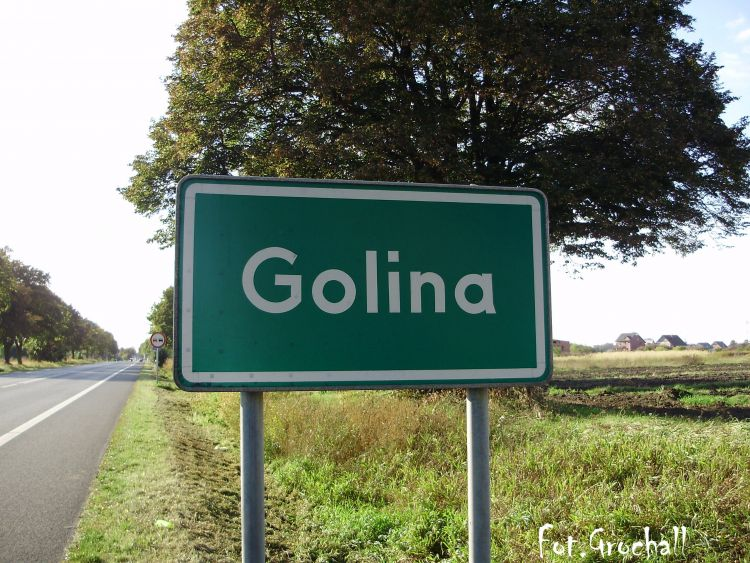
\includegraphics[scale=0.25]{golinatlo.jpg}
}
\quad
\subfigure[Obraz po wykryciu krawędzi]{
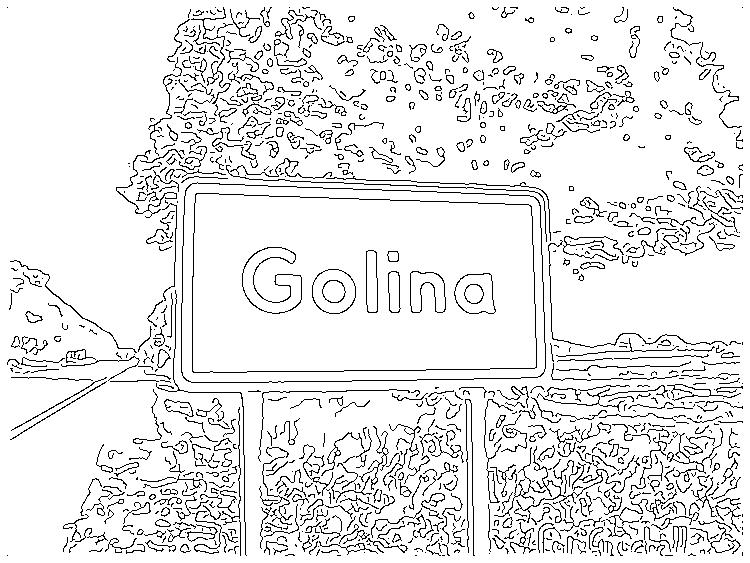
\includegraphics[scale=0.25]{golinacanny.jpg}
}
\renewcommand\figurename{Przykład}
\caption{Wynik wykrywania krawędzi detektorem Canny\\ 
źródło: opracowanie własne}
\end{figure}
\chapter{Architektura systemu}
Program został napisany, korzystając z obiektowości języka Java. Wykorzystano klasy oraz aktywności, które wzajemnie ze sobą powiązano, w celu minimalizacji ilości kodu, a także elastyczności kodu na zmiany. Diagram klas został przedstawiony na Rysunku 3.1. Wykonany został darmowym narzędziem $creatly$.
\begin{figure}[htbp]
\centering
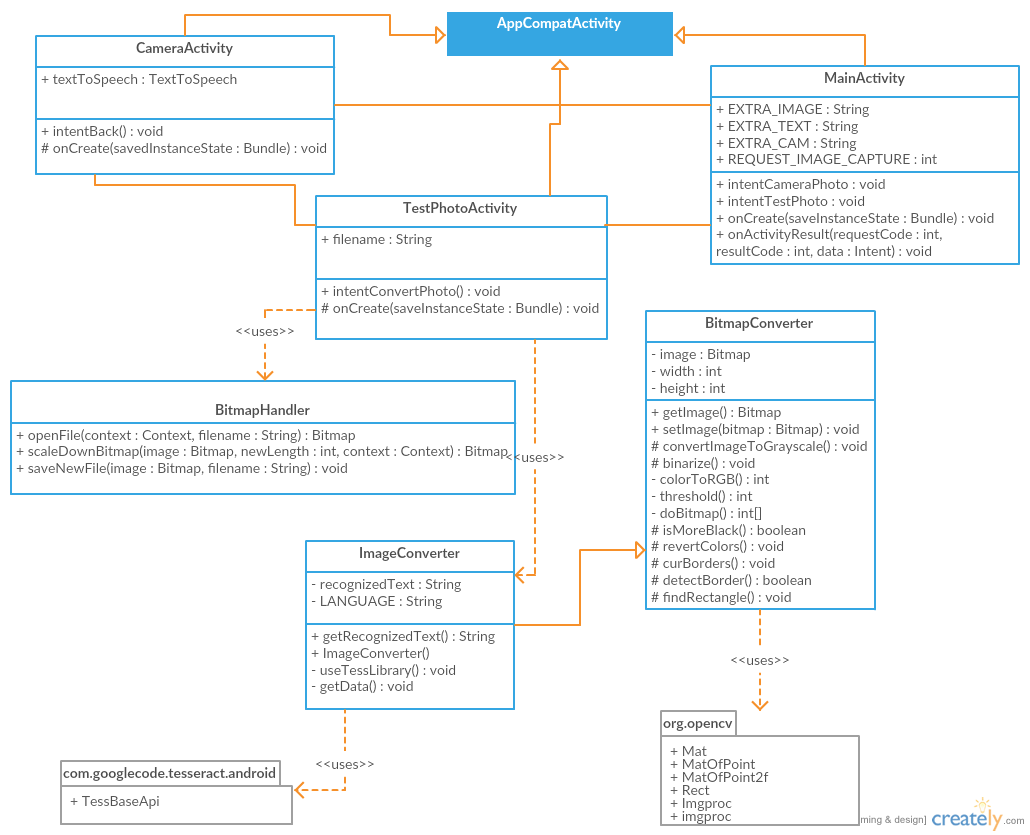
\includegraphics[scale=0.49]{diagramuml.png}
\caption{Diagram UML klas
\\ 
źródło: opracowanie własne}
\end{figure}

\par Komunikacja między Aktywnościami została zaimplementowana, korzystając z intencji, pojęcia te zostały wyjaśnione w paragrafie 4.1.2. Poniżej zostanie zcharakteryzowana każda z klas i Aktywności:
\begin{itemize}
\item \textbf{AppCompatActivity} to klasa bazowa, używana w przypadku Aktywności, które korzystają z dodatkowych bibliotek. Wchodzi w skład podstawowych bibliotek systemu Android \cite{appcompat}. 
\item \textbf{MainActivity} to Aktywność, która dziedziczy po \textbf{AppCompatActivity}. Obsługuje Widok główny aplikacji, zaprezentowany na rysunku 5.1. Składa się z dwóch obiektów typu $Button$, które przekierowują do dwóch różnych Widoków. Jeden jest obsługiwany przez kolejną Aktywność - \textbf{TestPhotoActivity} i zostanie opisany później, a drugi - kamera urządzenia mobilnego, jest również obsługiwany przez \textbf{MainActivity}. W Intencji, zrobione zdjęcie przesyłane jest do funkcji $onActivityResult$, gdzie zostaje odpowiednio przetworzone, tekst zostaje rozpoznany i w kolejnej Intencji wyniki tych dwóch operacji zostają przesłane do \textbf{CameraActivity}.
\item \textbf{TestPhotoActivity} to Aktywność, która również dziedziczy po \textbf{AppCompatActivity}. Zajmuje się obsługą Widoku testowego, wyświetla obiekty typu $ImageButton$, które po kliknięciu przesyłają Intencję z odpowiednim obrazem, który ma zostać poddany przetwarzaniu. Widok ten jest przedstawiony na rysunku 5.2. Przetworzony obraz wraz z rozpoznanym tekstem zostają przesłane do \textbf{CameraActivity}.
\item \textbf{CameraActivity} to Aktywność, która także dziedziczy po \textbf{AppCompatActivity}. Zajmuje się obsługą Widoku, który reprezentuje końcowy wynik działania aplikacji. Widok ten można znaleźć na rysunkach 5.3b, 5.4b oraz 5.5b. Sam Widok zawiera obiekty: $ImageView$, służący do wyświetlenia przetworzonego obrazu, $TextView$, służący do wyświetlenia odczytanego tekstu, oraz dwa obiektu typu $Button$, gdzie jeden przekierowuje użytkownika do poprzedniego Widoku, a drugi pozwala na powtórzenie komunikatu głosowego, który jest odczytywany z przekazanego do aktywności tekstu. W klasie odczytywana jest Intencja przesłana z Aktywności \textbf{MainActivity}, pobierany jest tekst, który rozpoznano na obrazie, typu String, następnie tekst ten zostaje odczytany, korzystając z klasy $TextToSpeech$, która została szerzej opisana w paragrafie 4.1.1.
\item \textbf{BitmapHandler} to klasa, która zajmuje się obsługą plików i bitmap. Konwertuje obraz w pliku do obiektu typu Bitmap w funkcji $openFile$. Zapisuje bitmapę do pliku w funkcji $saveNewFile$. Daje też możliwość przeskalowania bitmapy do mniejszego rozmiaru w funkcji $scaleDownBitmap$, co jest przydatną rzeczą, o tyle, o ile Android jest systemem, który jest w stanie sobie poradzić z obróbką większych obrazów, to już aby je wyświetlić, rozmiarowo należy dopasować je do ekranu urządzenia mobilnego na którym działa aplikacja.
\item \textbf{BitmapConverter} to klasa, która zajmuje się zasadniczą trudnością niniejszego projektu - przetwarza bitmapę w taki sposób, aby biblioteka Tess4j poradziła sobie z rozpoznaniem na niej tekstu. Wykorzystuje w tym celu bibliotekę OpenCV, a także własne, zaimplementowane funkcje. Na początek wycina ze zdjęcia prostokąt, przyjmując, że jest on znakiem drogowym, korzystając z funkcji $findRectangle$, której działanie zostało opisane w paragrafie 4.3.1. Kolejno prostokąt zostaje poddany operacjom: 
\begin{enumerate}
\item Przetworzenia do skali szarości w funkcji $convertImageToGrayscale$, korzystając z metody Jasność, opisanej w paragrafie 2.1.
\item Progowania metodą Otsu w funkcji $binarizeImage$, metoda ta została opisana w paragrafie 2.2.1.
\item Sprawdzenia czy jest więcej koloru czarnego na obrazie w funkcji $isMoreBlack$ i odwrócenia kolorów w funkcji $revertColors$, gdy czarny kolor występuje częściej, korzystając z założenia, że jeżeli chce się otrzymać czarny tekst na białym tle, to procentowo białe tło składa się z większej liczby pikseli. Problem, wraz z rozwiązaniem, szerzej opisany w paragrafie 4.4.
\item Sprawdzenia czy obraz jest obramowany w funkcji $detectBorders$. I jeżeli jest to pozbycie się tych obramowań w funkcji $cutBorders$. Obie funkcje szerzej opisane w paragrafie 4.4.
\end{enumerate}
\item \textbf{ImageConverter} to klasa, która dziedziczy po \textbf{BitmapConverter} i korzysta z biblioteki Tess4j. Konstruktor tej klasy wykonuje całe przetwarzanie obrazu i rozpoznanie tekstu. Przyjmuje zdjęcie w formacie Bitmap, wykonuje wszystkie operacje opisane we wcześniejszym punkcie, następnie przetwarza wynikową bitmapę na tekst i ten tekst jest wartością zwracaną konstruktora. Klasa ta powstała w celu rozdzielenia metod przetwarzających bitmapę i tych związanych z rozpoznawaniem tekstu. Zmniejszyła także liczbę komend wywoływanych w Intencjach, przesyłanych do Widoku z wynikiem działania aplikacji. W Intencjach inicjalizuje się jedynie obiekt klasy, korzystając z konstruktora. Obiekt ten składa się z przetworzonego obrazu i rozpoznanego tekstu.
\end{itemize}
\par Działanie programu można podzielić na kilka etapów, jak na Rysunku 3.2, przedstawiającym diagram przypadków użycia. Został on wykonany, korzystając z aplikacji $creatly$. Mamy: wejście, obsługę pliku, wykrywanie prostokątów, operacje na bitmapie oraz wyjście. Zaczynając od wejścia, pojawiają się dwie opcje w zależności od typu aktora, użytkownik będzie chciał zrobić zdjęcie obiektowi znajdującym się przed nim, więc wybierze opcję "Zrób zdjęcie", natomiast tester będzie chciał przetestować działanie aplikacji na znanych mu danych testowych, dlatego wybierze opcję "Wybierz zdjęcie". Kolejno wybrane zdjęcie będzie musiało zostać pobrane z pliku, następnie program zajmie się wykrywaniem prostokątów, zdjęcie z kamery od razu trafia do tego bloczka. Tutaj uczestniczy aktor, którym jest biblioteka OpenCV. Następnie prostokąty są odpowiednio przetwarzane wcześniej opisanymi operacjami na bitmapie. Dalej rozpoznaje się tekst, w czym uczestniczy aktor: Tess4j, i na urządzeniu mobilnym wyświetla się przetworzony obraz, a tekst zostaje przeczytany.
\begin{sidewaysfigure}[htbp]
\centering
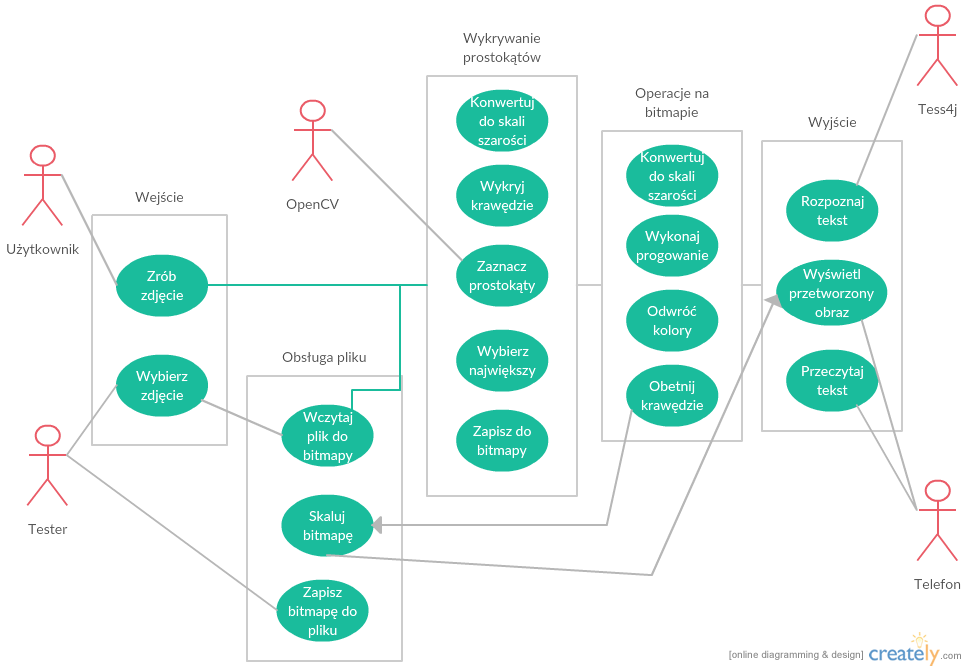
\includegraphics[scale=0.6]{usecasediagram.png}
\caption{Diagram UML przypadków użycia
\\ 
źródło: opracowanie własne}
\end{sidewaysfigure}
\chapter{Implementacja}
Projekt został napisany pod system operacyjny Android, a stworzony na platformie Android Studio, w związku z czym językiem implementacji była Java. W niniejszej pracy wykorzystano dwie otwarte, darmowe biblioteki dla platformy Java: Tess4j oraz OpenCV. Tess4j - bibliteka OCR, przetwarzała obraz na mowę, a z biblioteki OpenCV, która oferuje bardzo dużo funkcji do przetwarzania obrazów wykorzystano funkcję wykrywającą na obrazie prostokąty. 
\section{System operacyjny Android}
Aplikacja została napisana pod system operacyjny Android, jako, że ma on największy procentowy skład na rynku telefonów - 85\% \cite{procenty}. Natywnym jeżykiem w jakim pisze się aplikacje na system operacyjny Android jest Java. Jednak istnieją platformy, które pozwalają pisać również w innych językach np. C\#, korzystając z Xamarin. Xamarin był wcześniej platformą niezależną, ale po wykupieniu przez firmę Microsoft został dodany jako nakładka do Visual Studio 2015 w Aktualizacji 2. Języki C\# i Java są do siebie bardzo podobne, działają nawet na ekwiwalentnych wirtualnych maszynach - Java na JVM(Java Virtual Machine), a C\# na .NET. Jeszcze kilka lat temu największym atutem Javy był fakt, że jest ona rozwiązaniem międzysystemowym, działającym zarówno na systemie Windows jak i Linux \cite{thinking}, jednak aktualne aktualizacje .NETowe sprawiły, że różnica ta się rozmyła. Jednakże w tej pracy zdecydowano się na język natywny aplikacji androidowych, czyli Javę, z uwagi na o wiele bogatszą dokumentację, zarówno w języku polskim i angielskim, a także znaczną liczbę kursów i artykułów pomocnych przy pisaniu kodu. Java jest językiem, który radzi sobie z tymi przeszkodami, z którymi nie radzą sobie języki skryptowe i jest jednym z najpopularniejszych takich języków. Radzi sobie z takimi problemami jak dostęp do baz danych, przetwarzanie rozproszone, programowanie wielowątkowe, a także sieciowe \cite{java}. Jako IDE wykorzystano oficjalne dla platformy - Android Studio. Pierwsze implementacje były pisane na platformie Intellij IDEA, aby ułatwić debuggowanie oraz testowanie kodu, które trwało tutaj zdecydowanie krócej niż na podłączonym urządzeniu tudzież wirtualnej maszynie. Android Studio jest produktem stworzonym przez tą samą firmę, w związku z czym migracja między tymi dwiema platformami była najrozsądniejszym rozwiązaniem.
\subsection{TextToSpeech - zamiana tekstu na mowę}
Do przeczytania tekstu - konwersji obiektu typu String na mowę - użyto klasy TextToSpeech, znajdującej się w bibliotece platformy Android. Instancja tej klasy, po odpowiedniej inicjalizacji, od razu odtwarza dźwięk, który czyta podany tekst. Odpowiednia inicjalizacja polega na zaimplementowaniu $TextToSpeech.OnInitListener$\cite{texttospeech}. Inicjalizacja instancji następuje wtedy kiedy zostaje ona wywołana. Ustawia się tam język w jakim użytkownik chce aby tekst został przeczytany. Wartość języka przechowuje się w zmiennej $locale$. W przypadku ustawienia wartości domyślnej, tekst powinien zostać przeczytany w języku jaki ustawiony jest na urządzeniu mobilnym na którym działa aplikacja. Do zmiennej $toSpeak$ zostaje przesłana wartość z Intencji - wynik działania Tess4j.

\begin{lstlisting}[caption={Kod programu, który odpowiada za przeczytanie tekstu z wykorzystaniem klasy TextToSpeech}]

TextToSpeech textToSpeech=new TextToSpeech(getApplicationContext(),
new TextToSpeech.OnInitListener() {
    @Override
    public void onInit(int status) {
        if(status != TextToSpeech.ERROR) {
            Locale locale = new Locale("pl","PL");
            textToSpeech.setLanguage(locale);
        }
     }
});

final String toSpeak = getIntent().getExtras().getString(MainActivity.EXTRA_TEXT);
textToSpeech.speak(toSpeak, TextToSpeech.QUEUE_FLUSH, null);
\end{lstlisting}

\subsection{Intencje i Aktywności - komponenty platformy Android}
\textbf{Aktywność}(ang. $Activity$) to pojedyncza, skondensowana funkcjonalność, jaką może wykonać użytkownik. Skoro praktycznie każda Aktywność jest związana z interakcją z użytkownikiem, więc klasa ta zajmuje się tworzeniem \textbf{Widoków}(ang. $View$) z interfejsem użytkownika, które ustawiane są za pomocą funkcji $setContenView(View)$, gdzie zmienna $View$ to Widok, który programista chce połączyć z daną Aktywnością \cite{activity}. Widok to klasa reprezentująca GUI, czyli graficzny interfejs użytkownika. Korzysta z interaktywnych komponentów jak $Button$, czyli obiekt, reagujący w momencie kiedy się go naciśnie, wykonując akcję opisaną w Aktywności połączonej z tym Widokiem \cite{view}. Widok może być określony w pliku XML lub zaprogramowany metodą $drag and drop$(z ang. $weź i upuść$) - pojedyncze komponenty są pobierane z biblioteki oferowanej przez środowisko Android Studio, i umiejscawiane w odpowiednich regionach na prostokątnym polu, imitującym ekran telefonu. Cechy owych komponentów, takie jak nazwa, położenie, zależności między pozostałymi komponentami i inne są również ustawiane, poprzez wybieranie wartości cech z listy lub wpisywanie ich do odpowiednich pól.
\par \textbf{Intencja}(ang. $Intent$) to kolejny komponent androidowej aplikacji, abstrakcyjny opis operacji, która ma zostać wykonana \cite{intents}. Umożliwia komunikację między aplikacjami, a także wewnątrz pojedynczej aplikacji - pomiędzy Aktywnościami. Intencje, przez pryzmat ich drugiej własności - komunikacji między Aktywnościami, wykorzystanej w tej pracy, można podzielić na dwa rodzaje \cite{android4devs}:
\begin{itemize}
\item \textbf{Jawne} - w konstruktorze Intencji, obiekt, który ma wykonać zadanie jest ściśle określony - nazwą jego klasy.
\item \textbf{Niejawne} - zadeklarowana jest konkretna akcja, ale nie jest powiedziane jaki komponent ma ją wywołać\cite{damianchodorek}.
\end{itemize}
\par Poniżej zaprezentowano działanie intencji, wykorzystane w niniejszym projekcie. W Kodzie źródłowym 4.2 nastąpiło jawne zadeklarowanie Intencji w Aktywności - \textbf{MainActivity} i będzie ona wykonana w Aktywności \textbf{CameraActivity}. W Kodzie źródłowym 4.3 do Intencji zostają dodane obiekty różnego typu - przetworzony obraz oraz rozpoznany tekst. W Kodzie źródłowym 4.4 Intencja zostaje wywołana. Następnie w Kodzie źródłowym 4.4 pokazano jak obsłużono Intencje w klasie \textbf{CameraActivity}. Funkcją $getIntent$ pobrano Intencję, a następnie wszystkie dodatkowe obiekty, które zostały do niej dołączone, odwołując się do klasy z której pochodzą zmienną typu String. 
\begin{lstlisting}[caption={Zadeklarowanie intencji}]
Intent intent = new Intent(this, CameraActivity.class);
\end{lstlisting}
\begin{lstlisting}[caption={Przekazanie obiektów różnego typu w intencji}]
extra.putParcelable(MainActivity.EXTRA_IMAGE, imageConverter.getImage());
extra.putString(MainActivity.EXTRA_TEXT, imageConverter.getRecognizedText());
intent.putExtras(extra);
\end{lstlisting}
\begin{lstlisting}[caption={Wywołanie intencji}]
startActivity(intent);
\end{lstlisting}
\begin{lstlisting}[caption={Obsługa intencji w klasie w którym ma zostać wykonana}]
imageView.setImageBitmap((Bitmap) getIntent().getExtras().getParcelable(MainActivity.EXTRA_IMAGE));
final String toSpeak = getIntent().getExtras().getString(MainActivity.EXTRA_TEXT);
\end{lstlisting}
\section{OCR - optyczne rozpoznawanie znaków}
OCR (ang. $Optical Character Recognition$) to system przetwarzania dokumentów w formie papierowej na tekst, w taki sposób, aby otrzymanym wynikiem były cyfrowe informacje gotowe do dalszego przetwarzania. Ten zbiór technik jest często wykorzystywany w biznesie, przechowywanie wszystkich dokumentów zajmuje wiele miejsca, po zamianie ich na postać cyfrową - miejsce jest zaoszczędzane, a dane gotowe do ewentualnej dalszej obróbki \cite{dokument}. OCR wykorzystywany jest także przy odczytywaniu tablic rejestracyjnych samochodów, w technikach stosowanych przez policję \cite{car}. W niniejszej pracy techniki OCR zostały zastosowane do odczytania z odpowiednio przetworzonego obrazu - tekstu, i zapisanie go w obiekcie typu String.
\subsection{Biblioteka Tess4j}
Tess4j to opensource'owa biblioteka. Jest to nakładka na Tesseract OCR API dla platformy Java. Język w jakim napisana jest biblioteka Tesseract to C++. Biblioteka ta umożliwia optyczne rozpoznawanie znaków (OCR) umieszczonych w plikach w formatach - TIFF, JPEG, GIR, PNG oraz BMP, wielostronicowe obrazy TIFF, a także dokumenty w formacie PDF \cite{tess4j}.
Poniżej została przedstawiona część kodu programu. Zostaje stworzony obiekt klasy $TessBaseAPI$, określa się miejsce w urządzeniu mobilnym, gdzie znajduje się folder $tessdata$ - z danymi uczącymi w języku polskim, jeżeli na urządzeniu ów folder się nie znajduje, zostaje on ściągnięty z repozytorium umieszczonym w sieci na platformie Github. Następnie rozpoczyna się działanie aplikacji funkcją $init$, gdzie podaje się ścieżkę do pliku z danymi uczącymi oraz język w jakim mają być rozpoznawane słowa. Kolejno do funkcji $setImage$ podaje się obraz w jednym ze wcześniej przytoczonych formatów. Obraz ten musi być odpowiednio przetworzony, gdyż biblioteka nie wykrywa miejsca położenia tekstu na zdjęciu:
\begin{itemize}
\item Tekst nie może być pisany ręcznie.
\item Tekst musi być w kolorze czarnym.
\item Tekst musi być umiejscowiony na białym tle.
\item Na obrazie może znajdować się tylko tekst.
\end{itemize}

\begin{lstlisting}[caption={Kod programu, odpowiadający za odwołanie  do zewnętrznego API Tess4j}]
TessBaseAPI baseApi = new TessBaseAPI();
baseApi.setDebug(true);
File tessdataFolder = new File(
Environment.getExternalStorageDirectory().getAbsoluteFile() + "/tessdata");
if (!tessdataFolder.exists()) {
    getData();
}
String path = String.valueOf(
Environment.getExternalStorageDirectory()) + "/";
baseApi.init(path, LANGUAGE);
baseApi.setImage(bitmap);
String recognizedText = baseApi.getUTF8Text();
baseApi.end();
\end{lstlisting}
\section{Biblioteka OpenCV}
Biblioteka OpenCV to zbiór funkcji wykorzystywanych przy przetwarzaniu obrazów, jest otwarta i darmowa oraz można z niej korzystać na różnych systemach, jak Mac OS X, Windows i Linux. Biblioteka ta została napisana w jeżyku C, ale korzystając z odpowiednich nakładek można ją stosować również w języku takim jak Java.
\par Obraz w bibliotece OpenCV jest traktowany jako macierz, przecięcia kolumn i wierszy opisują położenie piksela i zawierają jego wartość, albo w postaci jednej liczby gdy obraz jest w skali szarości, albo w postaci trzech liczb, gdy obraz jest kolorowy. Wystpuje kilka typów zapisu danych Arr, Scalar i Mat. Ten ostatni został wykorzystany w niniejszej pracy \cite{opencv}.
\subsection{Wykrywanie prostokątów}
W celu użycia metody $boundingRect$, która wykrywa prostokąty na obrazie należało odpowiednio przygotować obraz wejściowy. Należało przetworzyć go do odcieni szarości, a następnie wyrysować jego krawędzie, metodą Canny. W poniższym kodzie tak przetworzony obraz znajduje się w zmiennej typu Bitmap o nazwie $converted$. Ze wszystkich wykrytych krawędzi, które tworzą obiekty przeanalizowano wszystkie te, które mają kształt prostokąta. Za każdym razem liczono pole wykrytej figury i sprawdzano czy jest większa od poprzedniego prostokąta. Korzystano z założenia, że znaki drogowe tekstowe mają kształt prostokątów i na zdjęciu zcentrowanym na taki znak, założono, że będzie on największym prostokątem. Następnie tworzy się nowy obiekt typu Bitmap o wymiarach znalezionego prostokąta i w wyniku działania poniższej funkcji otrzymuje się obiekt zawierający jedynie prostokąt, czyli w domniemaniu znak drogowy, gotowy do dalszej obróbki. Prostokąt ten jest wycięty z oryginalnego zdjęcia, z uwagi na to, że skorzystanie z detektora Canny o dużej rozpiętości progów zarysowało najważniejsze krawędzie, ale mogło zignorować napisy.
\begin{lstlisting}[caption={Kod programu, odpowiadający za wykrycie prostokątów przy użyciu biblioteki Open CV}]
List<MatOfPoint> contours = new ArrayList<MatOfPoint>();
Imgproc.findContours( converted, contours, new Mat(), Imgproc.RETR_LIST,Imgproc.CHAIN_APPROX_SIMPLE);
MatOfPoint2f approximateCurve = new MatOfPoint2f();
Bitmap bitmap = null;
int max = 0;
Mat copyMat = new Mat();
   for (int i=0; i<contours.size(); i++) {
       MatOfPoint2f contour2f = new MatOfPoint2f( contours.get(i).toArray() );
       double approximateDistance = Imgproc.arcLength(contour2f, true)*0.02;
       Imgproc.approxPolyDP(contour2f, approximateCurve, approximateDistance, true);
       MatOfPoint points = new MatOfPoint( approximateCurve.toArray() );
       Rect rectangle = Imgproc.boundingRect(points);

		if (rectangle.area() > max) {
	   		Rect newRectangle = new Rect(rectangle.x, rectectangle.y, rectangle.width, rectangle.height);
    		bitmap = Bitmap.createBitmap(rectangle.width, rectangle.height, Bitmap.Config.ARGB_8888);
    		copyMat = new Mat(mat, newRectangle); // mat - oryginalny obraz w formacie Mat
			max = rectangle.area();
        }
    }
Utils.matToBitmap(copy, bitmap);
image = bitmap;
}
\end{lstlisting}
\section{Przetwarzanie wykrytego prostokąta}
Jak wcześniej wspomniano wykryty prostokąt, z tekstowym znakiem drogowym, zostaje wycięty z oryginalnego zdjęcia, co znaczy, że jest to obraz, wciąż nie przetworzony. Należy go przetransformować do skali szarości i poddać progowaniu. Kolejne operacje są już ściśle związane ze specyfiką aplikacji. Z uwagi na konkretne cechy jakie musi mieć obraz, który będzie obsługiwany przez bibliotekę Tess4j sprawdza się, czy posiada on więcej koloru czarnego niż białego, zakłada się, że aby tekst był koloru czarnego, a tło koloru białego, to właśnie białych pikseli musi być więcej. Do tego celu wykorzystano funkcję $isMoreBlack$, której implementację przedstawiono w Kodzie źródłowym 4.8. Wylicza ona liczbę pikseli czarnych i białych, a następnie sprawdza, których jest więcej.
\begin{lstlisting}[caption={Kod programu, odpowiadający za sprawdzenie czy jest więcej czarnych pikseli}]
int blackCounter = 0;
int whiteCounter = 0;

for (int i = 0; i < image.getHeight(); i++) {
     for (int j = 0; j < image.getWidth(); j++) {
          int value = image.getPixel(j, i);
          if (value == Color.BLACK) {
              blackCounter++;
          } else {
              whiteCounter++;
          }
    }
}
    if (blackCounter > whiteCounter)
        return true;
    else return false;
\end{lstlisting}
\par Jeżeli powyższa funkcja zwróci wartość $true$, należy odwrócić kolory w obrazie, w programie zajmuje się tym funkcja $revertColors$ zaprezentowana w Kodzie źródłowym 4.9.
\begin{lstlisting}[caption={Kod programu, odpowiadający za odwrócenie kolorów w obrazie}]
Bitmap reverted = Bitmap.createBitmap(width, height, image.getConfig());

for (int i = 0; i < height; i++) {
     for (int j = 0; j < width; j++) {
          int value = image.getPixel(j, i);
          if (value == Color.BLACK) {
              reverted.setPixel(j, i, Color.WHITE);
          } else {
              reverted.setPixel(j, i, Color.BLACK);
          }
    }
}
image = reverted;
\end{lstlisting}
\par Część znaków tekstowych drogowych znajdujących się na ulicach posiada też obwódkę, która czasem powoduje, że biblioteka Tess4j nie jest w stanie wykryć tekstu znajdującego się na znaku. Dlatego napisano funkcję, która sprawdza czy owa obwódka istnieje. Jest to funkcja $detectBorded$, której kod źródłowy został przedstawiony pod numerem 4.10.
\begin{lstlisting}[caption={Kod programu, odpowiadający za sprawdzenie czy wykryty prostokąt otoczony jest obwódką w innym kolorze}]
for (int i = 1; i < height*0.1; i++) {
    for (int j = 1; j < width; j++) {
         if (image.getPixel(j, i) != image.getPixel(j-1,i-1))
             return true;
    }
}
return false;
\end{lstlisting}
\par W przypadku gdy funkcja $detectBorder$ zwróci wartość $true$, obraz zostaje wycięty w taki sposób, aby obwódki się pozbyć. Po analizie znaków drogowych tekstowych, określone przedziały procentowe znaku w jakich obwódka może występować i na podstawie tych badań napisano funkcję $cutBorder$, Kod źródłowy 4.11.
\begin{lstlisting}[caption={Kod programu, odpowiadający za obcięcie obrazu o konkretną procentową wartość}]
int borderWidth = (int) (0.05*width);
int borderHeight = (int) (0.05*height);
int newWidth = width - 2*borderWidth;
int newHeight = height - 2*borderHeight;
Bitmap imageWithoutBorders = Bitmap.createBitmap(newWidth, newHeight, image.getConfig());
int i_b = 0;
for (int i = borderHeight; i < newHeight+borderHeight; i++) {
     int j_b = 0;
     for (int j = borderWidth; j < newWidth+borderWidth; j++) {
          imageWithoutBorders.setPixel(j_b++, i_b, image.getPixel(j, i));
     }
     i_b++;
}
image = imageWithoutBorders;
\end{lstlisting}
\chapter{Działanie aplikacji i testy}
\section{Wymagania wstępne}
Aplikacja działa na smartfonach z oprogramowaniem Android o wersji SDK nie starszej niż 17. Wersją najbardziej oczekiwaną jest wersja 23. Smartfon musi posiadać aparat oraz ponad 13Mb wolnej pamięci – zostanie na niej zapisany folder – tessdata, z plikiem zawierającym dane potrzebne bibliotece Tess4j do przetwarzania obrazu w języku polskim. Język telefonu powinien być ustawiony na ten w jakim oczekiwane jest czytanie komunikatów przez aplikację. Poniżej zawarto zrzuty ekranu robione urządzeniem mobilnym na którym działała aplikacja.
\section {Widok główny}
\begin{figure}[htbp]
\centering
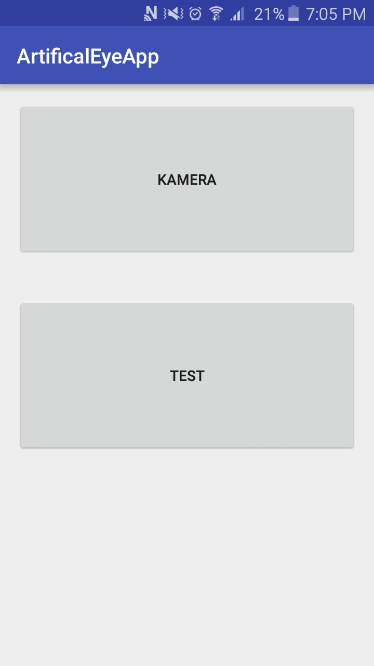
\includegraphics{glownywidok.png}
\renewcommand\figurename{Przykład}
\caption{Główny widok aplikacji
\\ 
źródło: opracowanie własne}\par\medskip

\end{figure}
Jest to intuicyjny Widok z dwoma dużymi przyciskami. Przy uruchomieniu aplikacji, informuje ona użytkownika komunikatem głosowym o położeniu przycisków i ich przeznaczeniu: „Kliknij na górze ekranu aby przejść do kamery – Kliknij na dole ekranu aby przejść do testów”. Aplikacja, poza Widokiem głównym, posiada dwa Widoki dodatkowe: użytkownika oraz testowy. Można się do nich dostać po wciśnięciu w odpowiedni przycisk. Przycisk „Kamera” przekierowuje użytkownika do widoku z kamery smartfona, natomiast przycisk „Test” przekierowuje do Widoku testowego.
\section{Widok docelowy}
Widok docelowy przenosi użytkownika do kamery zainstalowanej na urządzeniu na którym działa aplikacja. W tym momencie użytkownik ma możliwość kliknięcia w ekran i zrobienia fotografii. W zależności od rodzaju telefonu, kamera może poprosić o potwierdzenie przesłania zdjęcia do dalszej przeróbki, o czym aplikacja poinformuje komunikatem głosowym, z dokładnym umiejscowieniem odpowiedniego przycisku na ekranie, zdjęcie też może zostać od razu przesłane.
\section {Widok testowy}
\begin{figure}[htbp]
\centering
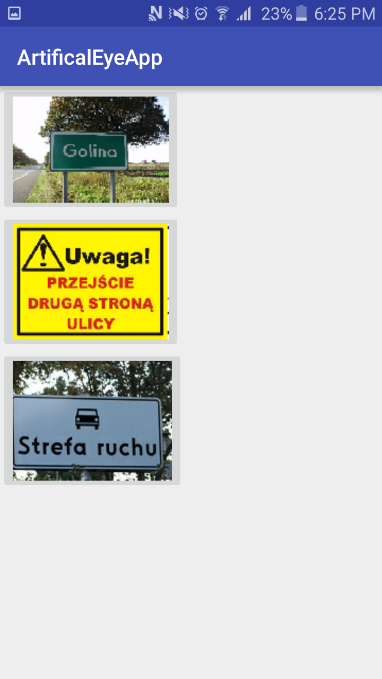
\includegraphics{widoktest.png}
\renewcommand\figurename{Przykład}
\caption{Testowy widok aplikacji
\\ 
źródło: opracowanie własne}\par\medskip

\end{figure}
\par Osoba testująca, klikając na wybrane zdjęcie sprawia, że zostaje ono poddane przetwarzaniu. W efekcie końcowym otrzymuje się rozpoznany znak, wycięty ze zdjęcia, jako obraz binarny – zaprezentowany przez dwa odcienie – czarny oraz biały, kolory odwrócone, odpowiednio tak aby tekst był czarny, a tło białe, czyli obraz jaki na wejście otrzymuje algorytm rozpoznający tekst. Pod obrazem zostaje wyświetlony tekst, którzy otrzymano w wyniku działania biblioteki Tess4j. Zostaje on przeczytany przez aplikację, użytkownik może odtwarzać go dowolną liczbę razy, klikając na przycisk „Powiedz”. Poniżej, na zdjęciach numer 5.3, 5.4 oraz 5.5, zostały przedstawione wyniki działania aplikacji w trybie testowym.
\begin{figure}
\centering
\subfigure[Obraz przetwarzany]{
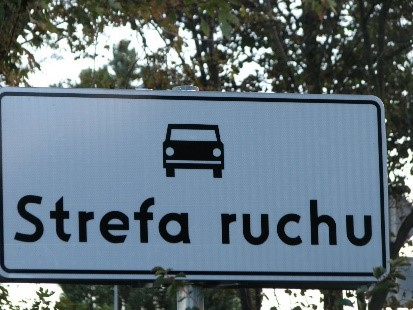
\includegraphics[scale=0.8]{strefaruchu.jpg}
}
\quad
\subfigure[Obraz przetworzony]{
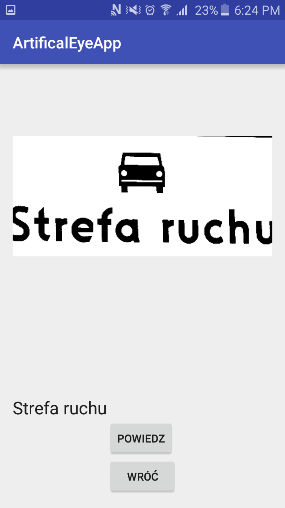
\includegraphics[scale=0.8]{strefaruchuwynik.png}
}
\renewcommand\figurename{Przykład}
\caption{Wynik działania aplikacji
\\ 
źródło: opracowanie własne}
\end{figure}
\\
\begin{figure}
\centering
\subfigure[Obraz przetwarzany]{

\includegraphics[scale=0.6]{uwaga.png}
}
\quad
\subfigure[Obraz przetworzony]{
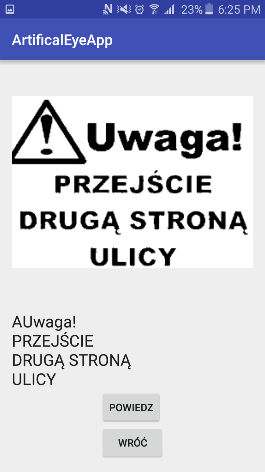
\includegraphics[scale=0.8]{uwagawynik.png}
}
\renewcommand\figurename{Przykład}
\caption{Wynik działania aplikacji\\ 
źródło: opracowanie własne}
\end{figure}

\begin{figure}
\centering
\subfigure[Obraz przetwarzany]{
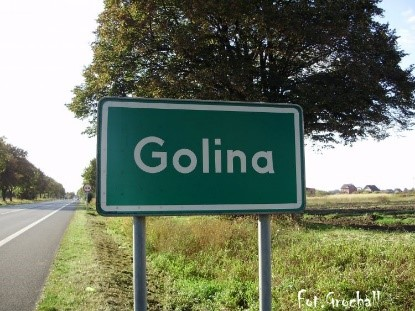
\includegraphics[scale=0.8]{golina.jpg}
}
\quad
\subfigure[Obraz przetworzony]{
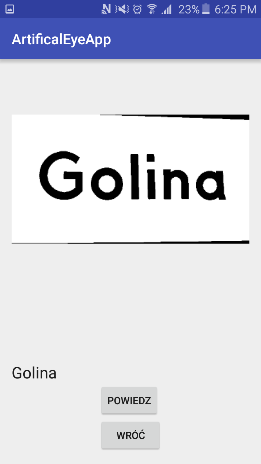
\includegraphics[scale=0.8]{golinawynik.png}
}
\renewcommand\figurename{Przykład}
\caption{Wynik działania aplikacji\\ 
źródło: opracowanie własne}
\end{figure}
\section{Testy}
Głównym problemem do rozwiązania było odpowiednie przetworzenie obrazu, aby biblioteka Tess4j sobie z nim poradziła. Testy zostały przeprowadzone w środwisku Intellij IDEA, a wyniki w postaci obrazów, zostały przedstawione poniżej.
\par Testowanie aplikacji zaczęto od najprostszych zdjęć znaków drogowych, gdzie wystarczyło je przekonwertować do skali szarości i poddać progowaniu, przykład przedstawiono na Przykładzie  5.6.
\begin{figure}[htbp]
\centering
\captionsetup{justification=centering}
\subfigure[Obraz przetwarzany]{

\includegraphics[scale=0.65]{rozbiorka.jpg}
}
\quad
\subfigure[Obraz przetworzony]{

\includegraphics[scale=0.55]{rozbiorkawynik.jpg}
}
\renewcommand\figurename{Przykład}
\caption{Wynik działania algorytmu przetwarzania obrazu\\ 
źródło: opracowanie własne}
\end{figure}
\par Kolejną napotkaną trudnością był fakt, że na znakach tekst nie zawsze jest ciemniejszy od tła, więc należało przetestować algorytm i na takich obrazach, przykład na Przykładzie 5.7.
\begin{figure}[htbp]
\centering
\captionsetup{justification=centering}
\subfigure[Obraz przetwarzany]{
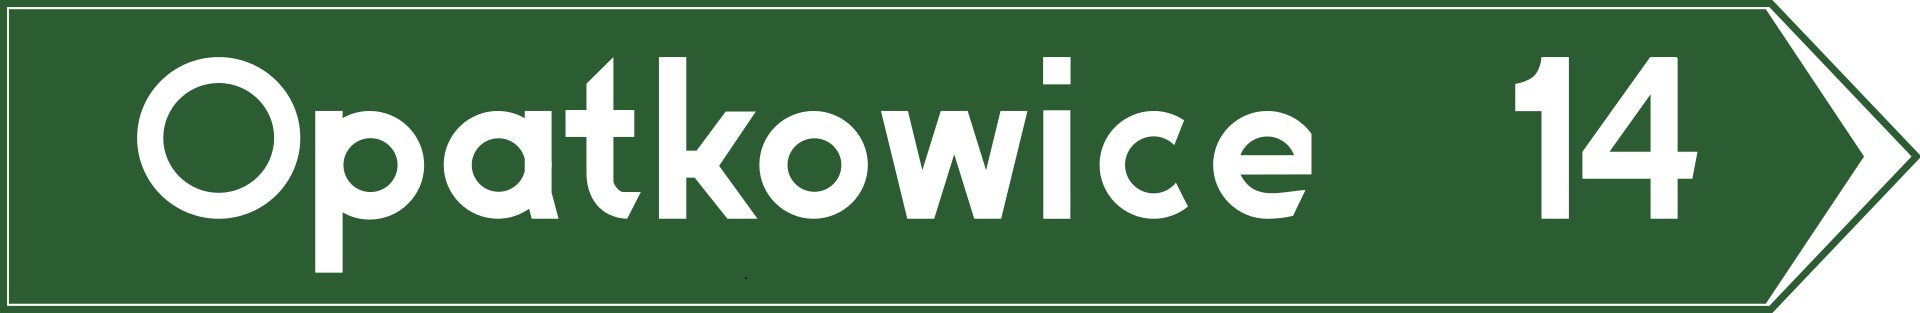
\includegraphics[scale=0.15]{opatkowice.jpg}
}
\quad
\subfigure[Obraz przetworzony]{

\includegraphics[scale=0.10]{opatkowicewynik.jpg}
}
\renewcommand\figurename{Przykład}
\caption{Wynik działania algorytmu przetwarzania obrazu\\ 
źródło: opracowanie własne}
\end{figure}
\par Kolejno wypróbowano algorytm na znakach, które posiadały więcej kolorów lub były otoczone tłem jak na Przykładzie 5.8.
\begin{figure}[htbp]
\centering
\captionsetup{justification=centering}
\subfigure[Obraz przetwarzany]{
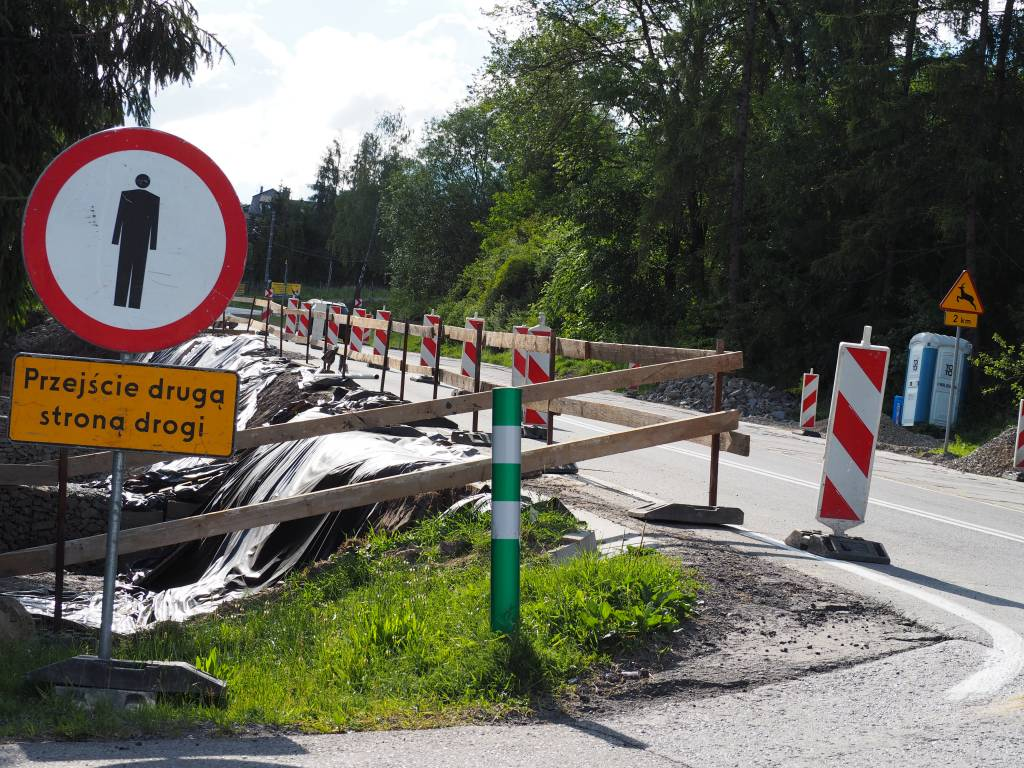
\includegraphics[scale=0.15]{drugastrona.JPG}
}
\quad
\subfigure[Obraz przetworzony]{
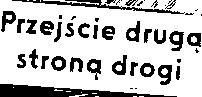
\includegraphics[scale=1]{drugastronawynik.jpg}
}
\renewcommand\figurename{Przykład}
\caption{Wynik działania algorytmu przetwarzania obrazu\\ 
źródło: opracowanie własne}
\end{figure} \newpage
\par Z uwagi na przyjęte założenia, dotyczące tego, że rozpoznawany znak jest zawsze największym prostokątem na zrobionej fotografii w przypadkach kiedy sąsiadują z nim inne znaki (Przykład 5.9), niekoniecznie tekstowe, algorytm zawodzi. 
\begin{figure}[htbp]
\centering
\captionsetup{justification=centering}
\subfigure[Obraz przetwarzany]{
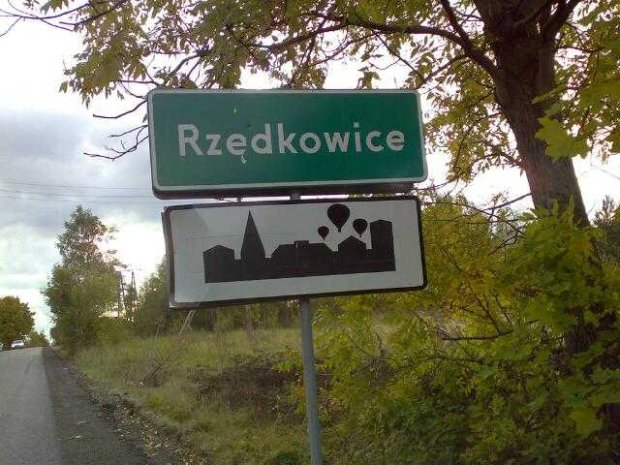
\includegraphics[scale=0.25]{rzedkowice.jpg}
}
\quad
\subfigure[Obraz przetworzony]{
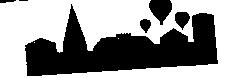
\includegraphics[scale=0.8]{rzedkowicewynik.jpg}
}
\renewcommand\figurename{Przykład}
\caption{Wynik działania algorytmu przetwarzania obrazu\\ 
źródło: opracowanie własne}
\end{figure}

\chapter{Podsumowanie}
Stworzona aplikacja i jej zaimplementowane funkcjonalności pokryły się z zamierzonym celem niniejszej pracy inżynierskiej. Środowisko Android Studio, w którym została napisana umożliwiło spełnienie wszystkich założeń projektowych, a także przeprowadzanie testów nie tylko na maszynie wirtualnej, ale również na urządzeniu mobilnym, czyli docelowym urządzeniu, na którym aplikacja ma pracować. Powstała prosta w obsłudze aplikacja, z interfejsem adekwatnym dla obranego użytkownika, jakim jest osoba niewidoma lub niedowidząca. Aplikacja ta korzysta z popularnych, prostych, ale skutecznych algorytmów przetwarzania obrazów, które zostały w powyższej pracy skrupulatnie opisane i przedstawione na tle innych możliwych rozwiązań, poza własną implementacją algorytmów, skorzystano także z dostępnych w sieci otwartych bibliotek - OpenCV oraz Tess4j. One również zostały omówione, przedstawiono ich zastosowania oraz przykładowe użycie.
\par Aplikacja jest napisana obiektowo, z możliwością rozszerzenia o kolejne funkcjonalności. Po prostu dodając kolejne Aktywności i Widoki. Napisano ją w języku Java, korzystając również z bibliotek natywnie napisanych w języku C++. Przy minimalnych zmianach, z uwagi na to, że biblioteki używane w Androidzie a te typowo związane z platformą Java, przy przetwarzaniu obrazów nieznacznie się różnią, aplikacja ta może pełnić funkcję aplikacji desktopowe do przetwarzania wczytanych obrazów na informację tekstową. Migracja programu na inne platformy, takie jak WindowsPhone, nie powinna być problematyczna ze względu na niebotyczne podobieństwo języków C\# oraz Java.
\begin{thebibliography}{99}
\bibitem{touch} HowStuffWorks: \emph{How BrailleTouch works} (dostęp: 3.12.2016)
\par URL:\hspace{0.1cm}http://electronics.howstuffworks.com/gadgets/other-gadgets/braille-touch.htm
\bibitem{rysunek} R. Tadeusiewicz, P. Korohoda: \emph{Komputerowa analiza i przetwarzanie obrazów}, Kraków: Wydawnictwo Fundacji Postępu Telekomunikacji, [1997] ('3)
\bibitem{obrazy} R. Tadeusiewicz, P. Korohoda: \emph{Komputerowa analiza i przetwarzanie obrazów}, Kraków: Wydawnictwo Fundacji Postępu Telekomunikacji, [1997] ('3)
\bibitem{wizja} jw. ('5)
\bibitem{grayscale} J.D. Cook: \emph{Converting color to grayscale} (dostęp: 3.12.2016) 
\par URL:\hspace{0.1cm}http://www.johndcook.com/blog/2009/08/24/algorithms-convert-color-grayscale
\bibitem{prog} Rafajłowicz E., Rafajłowicz W.: \emph {Wstęp do przetwarzania obrazów przemysłowych}, Wrocław : Oficyna Wydawnicza Politechniki Wrocławskiej, [2010]. ('82) 
\bibitem{histogram1} Wikipedia: \emph{Histogram} (dostęp: 3.12.2016) 
\par URL: https://pl.wikipedia.org/wiki/Histogram
\bibitem{histogram} jw. ('83-'84)
\bibitem{dwaprogi} jw. ('85)
\bibitem{auto} jw. ('85)
\bibitem{binaryzacja} \emph{IEEE Transactions on systems, man, and cybernetics}, vol. smc-9, no. 1, [1979] (dostęp: 3.12.2016)
\par URL: http://web-ext.u-aizu.ac.jp/course/bmclass/documents/otsu1979.pdf
\bibitem{krawedz} R. Jain, R. Kasturi, B. G. Schunck, \emph{Machine Vision} McGraw-Hill, Inc., edycja 1, [1995] ('140)
\bibitem{etapy} jw. ('145-146)
\bibitem{gauss} \emph{Gaussian Smoothing} (dostęp: 3.12.2016) 
\par URL: http://homepages.inf.ed.ac.uk/rbf/HIPR2/gsmooth.htm
\bibitem{appcompat} Android Developers: \emph{AppCompatActivity} (dostęp: 3.12.2016)
\par URL: https://developer.android.com/reference/android/support/v7/app/AppCompatActivity.html
\bibitem{procenty} \emph{Porównanie mobilnych systemów Android, iOS i Windows Phone 8} (dostęp: 3.12.2016) 
\par URL: http://www.benchmark.pl/testy\_i\_recenzje/android-ios-windows.html
\bibitem{thinking} B. Eckelo: \emph{Thinking in Java edycja polska}, Gliwice: Helion, wydanie 4, [2006] .  ('63-'64)
\bibitem{java} jw. ('62)
\bibitem{texttospeech} Android Developers: \emph{TextToSpeech} (dostęp: 3.12.2016) 
\par URL: https://developer.android.com/reference/android/speech/tts/TextToSpeech.html
\bibitem{activity} Android Developers: \emph{Activity} (dostęp: 3.12.2016) 
\par URL: https://developer.android.com/reference/android/app/Activity.html
\bibitem{view} Android Developers: \emph{View} (dostęp: 3.12.2016) 
\par URL: https://developer.android.com/reference/android/view/View.html
\bibitem{intents} Android Developers: \emph{Intent} (dostęp: 3.12.2016) 
\par URL: https://developer.android.com/reference/android/content/Intent.html
\bibitem{android4devs} android4devs: \emph{Wstęp do Intencji (Intents)} (dostęp: 3.12.2016 )
\par URL: http://www.android4devs.pl/2011/07/wstep-do-intencji-intents/
\bibitem{damianchodorek} Damian Chodorek: \emph{Kurs Android (5)} (dostęp: 3.12.2016) 
\par URL:\hspace{0.1cm}http://damianchodorek.com/2015/02/12/kurs-android-intent-intencje-komunikacja-aktywnosci-5
\bibitem{dokument} \emph{The role of OCR in invoice processing} (dostęp: 3.12.2016)
\par URL:\hspace{0.1cm}http://smart-soft.net/support/articles/automated-invoice-processing/the-role-of-ocr-in-invoice-processing.htm
\bibitem{car} Wikipedia: \emph{Automatic number plate tecognition} (dostęp: 3.12.2016)
\par URL: http://en.wikipedia.org/wiki/Automatic\_number\_plate\_recognition
\bibitem{tess4j} \emph {Tess4J - JNA wrapper for Tesseract} (dostęp: 3.12.2016)
\par URL: http://tess4j.sourceforge.net/
\bibitem{opencv} E. Rafajłowicz, W. Rafajłowicz, A. Rusiecki: \emph{Algorytmy przetwarzania obrazów i wstęp do pracy z biblioteką OpenCV}, Wrocław: Oficyna Wydawnicza Politechniki Wrocławskiej, [2010], ('23-'27)

\end{thebibliography}
\end{document}